% Format teze zasnovan je na paketu memoir
% http://tug.ctan.org/macros/latex/contrib/memoir/memman.pdf ili
% http://texdoc.net/texmf-dist/doc/latex/memoir/memman.pdf
% 
% Prilikom zadavanja klase memoir, navedenim opcijama se podešava 
% veličina slova (12pt) i jednostrano štampanje (oneside).
% Ove parametre možete menjati samo ako pravite nezvanične verzije
% mastera za privatnu upotrebu (na primer, u b5 varijanti ima smisla 
% smanjiti 
\documentclass[12pt,oneside]{memoir} 

% Paket koji definiše sve specifičnosti master rada Matematičkog fakulteta
\usepackage[latinica]{matfmaster} 
%
% Podrazumevano pismo je ćirilica.
%   Ako koristite pdflatex, a ne xetex, sav latinički tekst na srpskom jeziku
%   treba biti okružen sa \lat{...} ili \begin{latinica}...\end{latinica}.
%
% Opcija [latinica]:
%   ako želite da pišete latiniciom, dodajte opciju "latinica" tj.
%   prethodni paket uključite pomoću: \usepackage[latinica]{matfmaster}.
%   Ako koristite pdflatex, a ne xetex, sav ćirilički tekst treba biti
%   okružen sa \cir{...} ili \begin{cirilica}...\end{cirilica}.
%
% Opcija [biblatex]:
%   ako želite da koristite reference na više jezika i umesto paketa
%   bibtex da koristite BibLaTeX/Biber, dodajte opciju "biblatex" tj.
%   prethodni paket uključite pomoću: \usepackage[biblatex]{matfmaster}
%
% Opcija [b5paper]:
%   ako želite da napravite verziju teze u manjem (b5) formatu, navedite
%   opciju "b5paper", tj. prethodni paket uključite pomoću: 
%   \usepackage[b5paper]{matfmaster}. Tada ima smisla razmisliti o promeni
%   veličine slova (izmenom opcije 12pt na 11pt u \documentclass{memoir}).
%
% Naravno, opcije je moguće kombinovati.
% Npr. \usepackage[b5paper,biblatex]{matfmaster}

% Pomoćni paket koji generiše nasumičan tekst u kojem se javljaju sva slova
% azbuke (nema potrebe koristiti ovo u pravim disertacijama)
\usepackage[latinica]{pangrami}

% Datoteka sa literaturom u BibTex tj. BibLaTeX/Biber formatu
\bib{references}

% Ime kandidata na srpskom jeziku (u odabranom pismu)
\autor{Ivan Ristović}
% Naslov teze na srpskom jeziku (u odabranom pismu)
\naslov{Kreiranje zajedničke AST apstrakcije za različite programske jezike}
% Godina u kojoj je teza predana komisiji
\godina{2020}
% Ime i afilijacija mentora (u odabranom pismu)
\mentor{doc. dr Milena \textsc{Vujošević-Janičić}\\ Univerzitet u Beogradu, Matematički fakultet}
% Ime i afilijacija prvog člana komisije (u odabranom pismu)
\komisijaA{dr Ana \textsc{Anić}\\ University of Disneyland, Nedođija}
% Ime i afilijacija drugog člana komisije (u odabranom pismu)
\komisijaB{dr Laza \textsc{Lazić}\\ Univerzitet u Beogradu, Matematički fakultet}
% Ime i afilijacija trećeg člana komisije (opciono)
% \komisijaC{}
% Ime i afilijacija četvrtog člana komisije (opciono)
% \komisijaD{}
% Datum odbrane (odkomentarisati narednu liniju i upisati datum odbrane ako je poznat)
% \datumodbrane{}

% Apstrakt na srpskom jeziku (u odabranom pismu)
\apstr{%
\pangrami
}

% Ključne reči na srpskom jeziku (u odabranom pismu)
\kljucnereci{TODO}

\begin{document}
% ==============================================================================
% Uvodni deo teze
\frontmatter
% ==============================================================================
% Naslovna strana
\naslovna
% Strana sa podacima o mentoru i članovima komisije
\komisija
% Strana sa posvetom (u odabranom pismu)
\posveta{TODO zahvalnica}
% Strana sa podacima o disertaciji na srpskom jeziku
\apstrakt
% Sadržaj teze
\tableofcontents*

% ==============================================================================
% Glavni deo teze
\mainmatter
% ==============================================================================

\chapter{Uvod}
\label{chp:Intro}

Apstraktno sintaksičko stablo (engl. \emph{abstract syntax tree}, skr. \emph{AST}) programa ima značajnu ulogu u procesu kreiranja izvršivog programa od izvornog koda. AST nastaje parsiranjem izvornog koda, kao rezultat apstrahovanja stabla parsiranja koje generiše \emph{parser}. Parser čita izvorni k\^od i pokušava da u njemu pronađe primene određenih pravila jezika čiji je k\^od dizajniran da parsira. Svaki programski jezik ima specifična sintaksna pravila pa su stoga i skupovi pravila (tzv. \emph{gramatike}) programskih jezika raznorodni, što se zatim prenosi i na generisana stabla parsiranja. Stablo parsiranja se apstrahuje tako što se iz njega izvuku samo bitne sintaksne a uklone neke tehničke informacije.

Ovakva apstrakcija se najpre koristi u semantičkoj analizi programa koju vrši prevodilac nakon faze parsiranja i provere sintaksne ispravnosti koda. Ukoliko program prođe semantičke provere, prelazi se na prevođenje istog u međureprezentaciju i fazu optimizacije. Nakon faze optimizacije sledi generisanje asemblerskog koda koji se zatim prevodi u mašinski k\^od.

AST, zbog svoje uloge u semantičkoj analizi, može poslužiti i za analizu programa pre samog prevođenja, kroz proces poznat pod nazivom \emph{statička analiza}. Posmatranje programa kroz AST pruža mogućnost za poređenje dva programa na apstraktnom nivou. Jedna primena ove ideje u okviru statičke analize može biti provera semantičke ekvivalentnosti. Provera semantičke ekvivalentnosti dva programa je neodlučiv problem u opštem slučaju, međutim pod određenim pretpostavkama koje pojednostavljuju problem moguće je dizajnirati algoritme koji daju smislene rezultate u praksi. Jedna od često korišćenih pretpostavki je pretpostavka sličnosti strukture dva programa. Interesantno, provera da li dva programa zadovoljavaju ovu premisu se može proveriti posmatranjem izgleda i sličnosti u strukturi na apstraktnom nivou --- problem koji se može rešiti primenom algoritama za rad sa stablima jer je u pitanju AST (ali i grafovima uopšte, jer je stablo specijalizacija grafa).

Iako veoma konceptualno moćan alat, AST je ipak specifičan za konkretni programski jezik s obzirom da nastaje od stabla parsiranja koje je usko vezano za gramatiku konkretnog programskog jezika. Motivacija za ovaj rad dolazi od nepostojanja opštih apstrakcija sintaksičkih stabala koje bi se mogle koristiti za analizu programa napisanih u različitim programskim jezicima. Iako je broj programskih jezika danas veoma veliki, u okviru iste programske paradigme jezici moraju implementirati koncepte koji su potrebni da bi se programiralo u toj paradigmi i ta zajednička svojstva se mogu iskoristiti za formiranje zajedničke apstrakcije. 

U ovom radu će biti predstavljena opšta AST apstrakcija za imperativne programske jezike, sa ciljem da se omogući zajednička apstraktna reprezentacija velikog broja imperativnih jezika, pa čak i onih koji pripadaju skript paradigmi. Njena upotreba će biti demonstrirana na problemu semantičke ekvivalentnosti dobijenih apstrakcija kroz naivni algoritam poređenja simboličkih promenljivih. Štaviše, na apstraktnom nivou nije važno od kog se programskog jezika dobio AST, što može imati primenu u procesu migracije na nove tehnologije.

Naravno, semantička ekvivalentnost se ne mora zasnivati na apstrahovanju programa, već se takođe često rešava spuštanjem na nivo međukoda između višeg programskog jezika i asemblera. U nekim slučajevima se može iči i do asemblera pa i mašinskog jezika. Ukoliko bi se posmatrali asemblerski ili mašinski kod, vršilo bi se poređenje kodova prilagođenih određenoj arhitekturi procesora. U ovom radu je odabran AST-zasnovan pristup, s obzirom na važnosti i značaj apstraktnih sintaksičkih stabala, ali i zbog nedostatka opštih apstrakcija.

U poglavlju \ref{chp:RelevantTerms} će biti opisani relevantni pojmovi potrebni za razumevanje rada uz akcenat na apstraktnim sintaksičkim stablima i procesu njihovog dobijanja. Opšta AST apstrakcija za imperativne jezike biće opisana u poglavlju \ref{chp:MyAST}, a njena upotreba u problemu odlučivanja semantičke ekvivalentnosti kao i sam algoritam za poređenje opštih apstrakcija biće opisani u poglavlju \ref{chp:ASTComparing}. Implementacija apstrakcije i algoritma semantičkog poređenja će biti opisana u poglavlju \ref{chp:Implementation}. Na kraju, biće dati glavni zaključci ovog rada kao i moguća unapređenja i budući koraci. 

\chapter{Pregled relevantnih pojmova}
\label{chp:RelevantTerms}

U ovom poglavlju će biti opisani koncepti i alati čije je razumevanje potrebno kako bi se razumeo opis dalje apstrakcije i implementacije samog programa. Umesto analize samog sadržaja izvornog koda analizira se \emph{apstraktno sintaksno stablo} (eng. \emph{Abstract Syntax Tree}, u daljem tekstu \emph{AST}), opisano u odeljku \ref{sec:AST}. Više reči o alatima koji mogu da od proizvoljne gramatike kreiraju leksere i parsere biće u \ref{sec:ParsingGrammars}, sa akcentom na alatu \emph{Another Tool For Language Recognition} \cite{ANTLR}, u daljem tekstu \emph{ANTLR}, opisan u odeljku \ref{sec:ANTLR}. Parser generiše AST specifičan za datu gramatiku i nema sličnosti u dobijenim apstrakcijama za različite jezike. Kako bismo poredili stabla različitih jezika, kreiramo reprezentaciju na višem nivou i specifični AST podižemo na taj nivo. Ta reprezentacija će biti opisana u narednim poglavljima, kao i načini kako se ona može analizirati. Takođe, pojmovi specifični za implementaciju će takođe biti opisani u ovom poglavlju.

\section{Apstraktna sintaksička stabla}
\label{sec:AST}

Kako bi se k\^od pisan u nekom programskom jeziku (\emph{izvorni fajl}) preveo u k\^od koji će se izvršavati na nekoj mašini (\emph{izvršivi fajl}), prevodilac izvršava određene korake. Prvi korak je prepoznavanje gradivnih elemenata programskog jezika koji se nazivaju \emph{lekseme}, nalik na prepoznavanje reči u rečenicama govornog jezika, i raspodela leksema u grupe po funkciji (nalik na funkcije reči u govornom jeziku --- subjekti, predikati, objekti itd.). Nakon prepozavanja leksema, proverava se da li niz prepoznatih leksema ispunjava pravila odnosno \emph{sintaksu} programskog jezika, nalik na proveru da li se složene govorne rečenice sastoje od subjekta i predikta u određenom redosledu. Na kraju se proverava značenje odnosno \emph{semantika} koda, nalik na proveru da li govorne rečenice, iako sintaksno pravilne, imaju smisla. Deo prevodioca koji određuje da li je izvorni k\^od ispravno formiran u terminima leksike, sintakse i semantike se naziva \emph{prednji deo} (engl. \emph{front end}). Ukoliko je izvorni k\^od ispravan, prednji deo kreira \emph{međureprezentaciju} koda (engl. \emph{intermediate representation}, u daljem tekstu \emph{IR}) nad kojom se vrše optimizacije koda i koja se koristi za dalji proces prevođenja. Ukoliko to nije slučaj, prevođenje ne uspeva i programeru se daje poruka sa obrazloženjem zašto prevođenje nije uspelo \cite{EngineeringCompilers}.

Za potrebe ovog rada, što se procesa prevođenja tiče, dovoljno je poznavanje pomenutih procesa koje izvodi prednji deo, stoga neće biti reči o ostalim koracima u fazi prevođenja (optimizovanje, generisanje IR). Zainteresovani čitalac može više detalja pronaći u \cite{DragonBook}, \cite{EngineeringCompilers} i \cite{CompilerConstruction}. 

Pretpostavimo da želimo da prevedemo izvorni k\^od pisan u programskom jeziku C sa slike \ref{fig:CompilationProcessInit}. Primetimo da postoji greška u datom kodu --- simbol \texttt{c} koji se koristi u dodeli u liniji $7$ će biti prepoznat kao identifikator koji ne odgovara nijednoj deklarisanoj promenljivoj --- stoga ne možemo prevesti ovaj k\^od. Ovo nije greška u sintaksi --- izraz \texttt{a+c} je validan u programskom jeziku C. Problem će postati vidljiv tek nakon parsiranja izvornog koda i provere ispunjenosti sintaksih pravila, tačnije u fazi semantičke provere. Stoga se ovakve greške nazivaju \emph{semantičke greške}, dok se greške u sintaksi nazivaju \emph{sintaksne greške}.

\begin{figure}[h!]
\begin{lstlisting}
#include<stdio.h>
#define T int

int main()
{
    T a, b;
    a = a + c;        // c nije deklarisano
    printf("%d", a);
    return 0;
}
\end{lstlisting}
\caption{Primer izvornog koda sa semantičkom greškom (C).}
\label{fig:CompilationProcessInit}
\end{figure}

Pre nego što prednji kraj prevodioca dobije k\^od koji treba da prevede u međureprezentaciju, vrši se \emph{pretprocesiranje} od strane programa koji se naziva \emph{pretprocesor}. U fazi pretprocesiranja se izvode samo tekstualne operacije kao što su brisanje komentara ili zamena makroa u jezicima kao što je C. Rezultat rada pretprocesora za izvorni k\^od sa slike \ref{fig:CompilationProcessInit} se može videti na slici \ref{fig:CompilationProcessPrep}\footnote{U nekim implementacijama C standardne biblioteke, moguće je da se poziv funckije \texttt{printf} zameni pozivom funkcije \texttt{fprintf} sa ispisom na \texttt{stdout}. U standardu se propisuje da funkcije kao što je \texttt{printf} mogu biti implementirane kao makroi. Izlaz na slici \ref{fig:CompilationProcessPrep} je generisan od strane \texttt{GCC 7.4.0} po C11 standardu i ovo nije slučaj u datom okruženju.}.

\begin{figure}[h!]
\begin{lstlisting}
# 1 "<stdin>"
# 1 "<built-in>"
# 1 "<command-line>"
# 31 "<command-line>"
# 1 "/usr/include/stdc-predef.h" 1 3 4

...

extern char *ctermid (char *__s) __attribute__ ((__nothrow__ , __leaf__));
# 840 "/usr/include/stdio.h" 3 4
extern void flockfile (FILE *__stream) __attribute__ ((__nothrow__ , __leaf__));
extern int ftrylockfile (FILE *__stream) __attribute__ ((__nothrow__ , __leaf__)) ;
extern void funlockfile (FILE *__stream) __attribute__ ((__nothrow__ , __leaf__));
# 868 "/usr/include/stdio.h" 3 4
# 2 "<stdin>" 2
# 2 "<stdin>"

int main()
{
    int a, b;
    a = a + c;
    printf("%d", a);
    return 0;
}
\end{lstlisting}
\caption{Prikaz rezultata rada pretprocesora za izvorni k\^od sa slike \ref{fig:CompilationProcessInit}. Pritom, prikazano je samo par linija sa početka i kraja izlaza pretprocesora --- k\^od iznad \texttt{main} funkcije je uključen iz \texttt{stdio.h} zaglavlja.}
\label{fig:CompilationProcessPrep}
\end{figure}

U toku faze leksičke analize, kako prevodilac ne bi radio nad sirovim karakterima izvornog koda, potrebno je izvršiti transformaciju karaktera izvornog koda. Prevodilac ima u vidu elemente programskog jezika i šablone za njihovo prepoznavanje. Lekseme su one sekvence karaktera izvornog koda koje zadovoljavaju ove šablone. Lekseme se dalje razvrstavaju u kategorije, tzv. \emph{tokene} --- ključne reči, operatore, promenljive itd. Proces dobijanja tokena od izvornog koda se naziva \emph{tokenizacija}. Komponenta prednjeg dela koja vrši tokenizaciju se naziva \emph{skener} ili \emph{lekser}. Pojednostavljen primer šablona koje lekser pokušava da prepozna se mogu videti na slici \ref{fig:CLexerExample}. Primer izlaza leksera za izlaz pretprocesora sa slike \ref{fig:CompilationProcessPrep} se može videti na slici \ref{fig:CompilationProcessLex}.

\begin{figure}[h!]
\begin{lstlisting}[language={}]
Identifier 
    : IdentifierNondigit (IdentifierNondigit | Digit)*
    ;
IdentifierNondigit  
    : Nondigit
    | UniversalCharacterName
    ;
Nondigit 
    : [a-zA-Z_]
    ;
Digit 
    : [0-9]
    ;
\end{lstlisting}
\caption{Primer delimične definicije tokena za ime promenljive po C11 standardu.}
\label{fig:CLexerExample}
\end{figure}

\begin{figure}[h!]
\begin{lstlisting}[language={}]
identifier 'main'	 [LeadingSpace]	Loc=<sample.c:3:5>
l_paren '('		Loc=<sample.c:3:9>
r_paren ')'		Loc=<sample.c:3:10>
l_brace '{'	 [StartOfLine]	Loc=<sample.c:4:1>
int 'int'	 [StartOfLine] [LeadingSpace]	Loc=<sample.c:5:5>
identifier 'a'	 [LeadingSpace]	Loc=<sample.c:5:9>
comma ','		Loc=<sample.c:5:10>
identifier 'b'	 [LeadingSpace]	Loc=<sample.c:5:12>
semi ';'		Loc=<sample.c:5:13>
identifier 'a'	 [StartOfLine] [LeadingSpace]	Loc=<sample.c:6:5>
equal '='	 [LeadingSpace]	Loc=<sample.c:6:7>
identifier 'a'	 [LeadingSpace]	Loc=<sample.c:6:9>
plus '+'	 [LeadingSpace]	Loc=<sample.c:6:11>
identifier 'c'	 [LeadingSpace]	Loc=<sample.c:6:13>
semi ';'		Loc=<sample.c:6:14>
identifier 'printf'	 [StartOfLine] [LeadingSpace]	Loc=<sample.c:7:5>
l_paren '('		Loc=<sample.c:7:11>
string_literal '"%d"'		Loc=<sample.c:7:12>
comma ','		Loc=<sample.c:7:16>
identifier 'a'	 [LeadingSpace]	Loc=<sample.c:7:18>
r_paren ')'		Loc=<sample.c:7:19>
semi ';'		Loc=<sample.c:7:20>
return 'return'	 [StartOfLine] [LeadingSpace]	Loc=<sample.c:8:5>
numeric_constant '0'	 [LeadingSpace]	Loc=<sample.c:8:12>
semi ';'		Loc=<sample.c:8:13>
r_brace '}'	 [StartOfLine]	Loc=<sample.c:9:1>
eof ''		Loc=<sample.c:9:2>
\end{lstlisting}
\caption{Proces tokenizacije koda sa slike \ref{fig:CompilationProcessPrep} (generisano pomoću kompajlera \texttt{clang} \cite{Clang}).}
\label{fig:CompilationProcessLex}
\end{figure}

Nakon faze skeniranja potrebno je proveriti da li niz pročitanih tokena zadovoljava sintaksu programskog jezika. Pevodilac stoga mora da uporedi strukturu koda sa unapred definisanom strukturom za određeni programski jezik što zahteva formalnu definiciju sintakse jezika. Programski jezik možemo posmatrati kao skup \emph{pravila} pod imenom \emph{gramatika} \cite{ContextFreeGrammars}. Na slici \ref{fig:CompilationProcessGram} se može videti deo gramatike programskog jezika C. Proces provere zadovoljenosti sintaksnih pravila se naziva \emph{parsiranje}, a komponenta prednjeg dela koja vrši parsiranje se naziva \emph{parser}.\footnote{Moderni kompajleri često nemaju odvojene faze skeniranja i parsiranja, već se skeniranje odvija paralelno sa fazom parsiranja. Međutim, to nas ne sprečava da ispišemo tokene onda kada se oni prepoznaju, što to je demonstrirano na slici \ref{fig:CompilationProcessLex}.}

\begin{figure}[h!]
\begin{lstlisting}[language={}]
declarationList
    :   declaration
    |   declarationList declaration
    ;
declaration
    :   declarationSpecifiers initDeclaratorList ';'
    | 	declarationSpecifiers ';'
    |   staticAssertDeclaration
    ;
\end{lstlisting}
\caption{Prikaz para pravila iz gramatike programskog jezika C po standardu C11.}
\label{fig:CompilationProcessGram}
\end{figure}

Parser, imajući u vidu gramatiku jezika, kreira \emph{stablo parsiranja} (eng. \emph{parse tree} ili \emph{derivation tree}). Takvo stablo i dalje sadrži sve relevantne informacije o izvornom kodu. Vizuelni prikaz rada parsera za gramatiku sa slike C11 i izvornog koda sa slike \ref{fig:CompilationProcessInit} je dat na slici \ref{fig:CompilationProcessPars}. Stablo parsiranja se koristi u narednim fazama prevođenja.

\begin{figure}[h!]
\centering
\scalebox{0.95}[1.3] {
    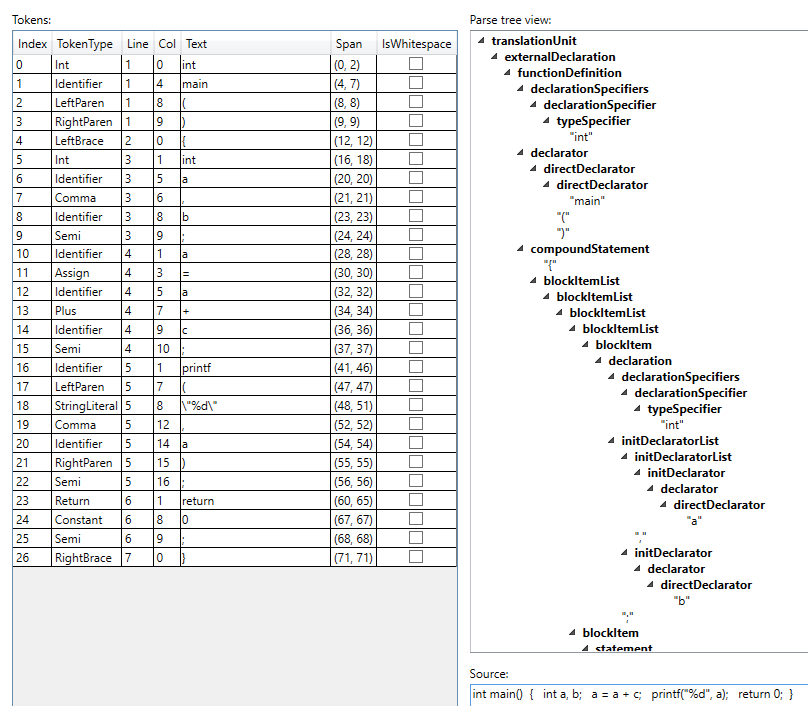
\includegraphics[width=\textwidth]{images/parse_tree.png}
}
\caption{Prikaz dela stabla parsiranja koje generiše parser kreiran od strane alata ANTLR4 \cite{ANTLR} za k\^od sa slike \ref{fig:CompilationProcessPrep}.}
\label{fig:CompilationProcessPars}
\end{figure}

Stablo parsiranja sadrži sve informacije potrebne u fazi parsiranja uključujući detalje korisne samo za parser prilikom provere ispunjenosti gramatičkih pravila. Sa druge strane, \emph{apstraktno sintaksičko stablo} sadrži samo sintaksičku strukturu u jednostavnijoj formi. Na slici \ref{fig:CompilationProcessPars1} se može videti koliko stablo parsiranja može biti kompleksno čak i za jednostavne aritmetičke izraze. Razlog kompleksnosti u ovom slučaju dolazi iz rekurzivnih pravila iz C11 gramatike. Parseru su sve ove informacije neophodne ali za naredne analize i proces prevođenja one nisu potrebne i zato se stablo parsiranja apstrahuje. Na primer, jedina važna semantička odlika izraza \texttt{a+c} je da je to zbir vrednosti nekih promenljivih. Na slici \ref{fig:ASTVariants} se mogu videti različita apstraktna sintaksička stabla za pomenuti izraz, ali takođe i za malo složenije izraze. Podrazumeva se, naravno, da je ulaz već tokenizovan. 

\begin{figure}[h!]
\centering
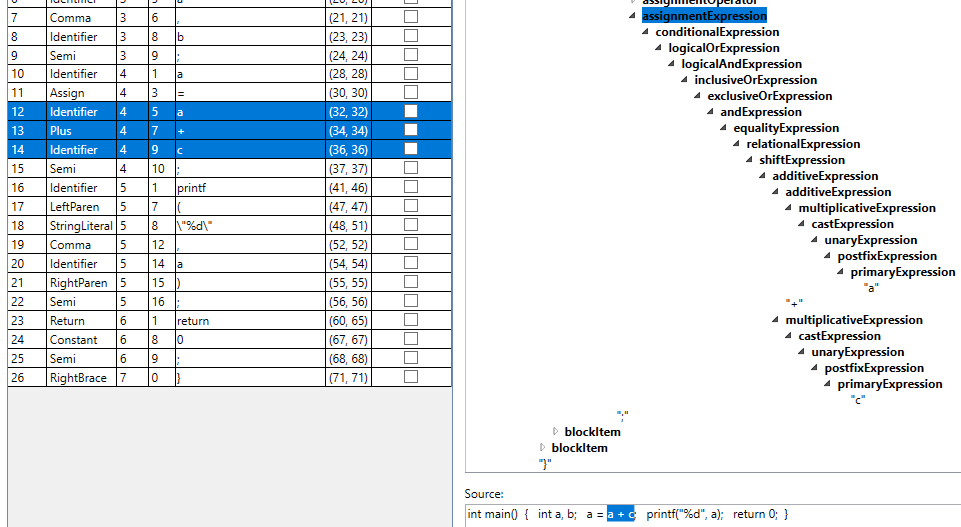
\includegraphics[scale=0.55]{images/parse_tree_expr.png}
\caption{Prikaz kompleksnosti stabla parsiranja za izraz 
\texttt{a+c} u C11 gramatici.} 
\label{fig:CompilationProcessPars1}
\end{figure}

\begin{figure}[h!]
\centering
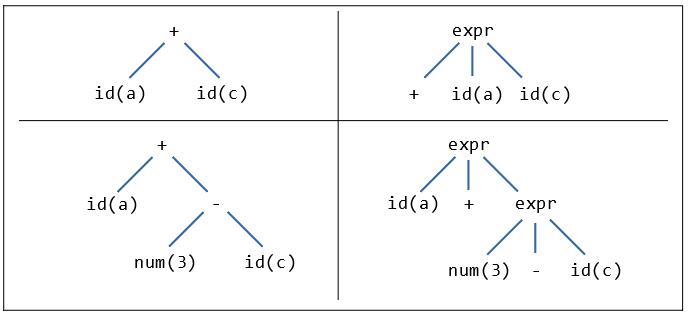
\includegraphics[scale=0.7]{images/ast.png}
\caption{AST varijante bez regularnosti (levo) i sa regularnošću (desno) za izraze \texttt{a+c} (gore) i \texttt{a+(3-c)} (dole).} 
\label{fig:ASTVariants}
\end{figure}

Uloga apstraktnog sintaksičkog stabla \cite{FormalSyntaxAndSemantics} je da pokaže semantiku strukture koda preko stabla. Kao što se vidi na slici \ref{fig:ASTVariants}, postoji određeni nivo slobode prilikom njihovog kreiranja. Generalno, \emph{terminalni simboli} --- simboli koji predstavljaju listove stabla parsera --- koji odgovaraju operatorima i naredbama se podižu naviše i postaju koreni podstabala, dok se njihovi operandi ostavljaju kao njihovi potomci u stablu. Desna stabla sa slike ne prate u potpunosti ovaj princip, ali se takođe koriste zbog regularnosti izraza --- ukoliko binarni izraz posmatramo kao apstrakciju, za implementaciju je lakše koristiti ovakav tip apstraktnih sintaksičkih stabala i stoga će biti korišćen kasnije u implementaciji opšte apstrakcije. Primetimo takođe da se u stablima za izraz \texttt{a+(3-c)} (dole) implicitno sačuvala informacija o prioritetu operacije oduzimanja u izrazu. Jasno je, dakle, da se računanje vrednosti aritmetičkih izraza onda vrši kretanjem od listova stabla ka korenu. Takođe, pošto je apstraktno sintaksičko stablo apstrakcija stabla parsiranja, više semantički ekvivalentnih izraza može imati isto apstraktno sintaksičko stablo ali različito stablo parsiranja; na primer, ako razmatramo izraz \texttt{(a+5)-x/2} i izraz \texttt{a+5-(x/2)}.


\section{Simboličko izračunavanje}
\label{sec:Symbolics}

Tokom procesa pronalaženja grešaka u radu softvera koriste se ručno pisani testovi i pregledi koda od strane drugih programera, i ove mere provere koda mogu verifikovati da softver, ili deo softvera, funkcioniše na različitim nivoima komplikovane arhitekture velikih projekata. Uprkos svim ovim merama, greške su i dalje nezaobilazne - jedan test može proveriti ponašanje koda za samo jedan ulaz. S obzirom da je nemoguće testirati sve moguće ulaze zbog njihovog ogromnog broja (ukoliko posmatramo samo funkciju jedne promenljive koja prima 32-bitni ceo broj, broj mogućih ulaza je $2^{32}$) nadamo se da testovi dobro \emph{generalizuju} - da pokrivaju opšte ali i neke specijalne ulaze. To se postiže uočavanjem da se vrednosti ulaza mogu razvrstati u klase po tome kakav izlaz uzrokuju. Ukoliko imamo funkciju koja treba da podeli dva broja, te klase mogu biti celi brojevi, realni brojevi, neke specijalne vrednosti specifične za to šta se testira (u ovom slučaju, $0$), kao i granice za tip podataka iz čijeg domena argumenti mogu uzeti vrednost. Čak i ovakav pristup, iako drastično smanjuje broj testova i eliminiše redundantne testove, i dalje zahteva relativno veliki broj testova u slučaju većih projekata i stoga je teško pronaći sve greške, pogotovo u slučajevima koji se retko dešavaju i zavise recimo od stanja drugih komponenti ili pak nekih nedeterminističkih ponašanja. U komplikovanim projektima je teško pokriti čitav izvorni kod testovima (engl. \emph{code coverage}) - iako pokrivenost koda od 100\% i dalje ne znači da taj kod ispravno radi.

\emph{Statička analiza koda} predstavlja analizu izvornog koda bez pokretanja istog. Ideja je baš ispitivanje svih mogućih stanja u kojima se može naći program i testiranje svih mogućih ulaza u jedinicu koja se testira. U praksi se nailazi na puno problema - osnovni je razlika simboličke i programerske apstrakcije. 

Simboličko izvršavanje \cite{SymbolicExecution} predstavlja sredinu između klasične verifikacije putem pisanja testova i statičke analize koda. Prilikom simboličkog izvršavanja, umesto stvarnih vrednosti ulaza koje se koriste u testovima, koriste se \emph{simboličke promenljive}. Simbolička promenljiva nije vezana za specifičnu vrednost i analiza se dalje vrši samo nad njom - samim tim se istovremeno mogu testirati višestruke klase sličnih ulaza. 

Primer simboličkog izvršavanja će biti opisan na isečku C sa slike \ref{fig:SymbolicExecCode}. Pretpostavimo da imamo deklarisanje promenljive \texttt{a}, \texttt{b} i \texttt{c} i da se neke operacije izvršavaju nad njima, reprezentovano komentarom. U nekom trenutku se vrednosti tih promenljivih koriste kao uslovi od kojih zavisi prolaznost testa u poslednjoj liniji. Dodelimo svakoj promenljivoj simboličku vrednost - \texttt{a = }$\alpha$, \texttt{b = }$\beta$, \texttt{c = }$\gamma$. Možemo izgraditi stablo izvršavanja i uslove koji moraju da važe nad simboličkim vrednostima $\alpha$, $\beta$ i $\gamma$ kako bi test u poslednjoj liniji prošao.

\begin{figure}[h!]
    \begin{lstlisting}[language={}]
    int a, b, c;

    // ...

    int x = 0; int y = 0; int z = 0;
    if (a)      
        x = -2;
    if (b < 5)  {
        if (!a && c)    
            y = 1;
        z = 2;
    }

    assert(x + y + z != 3);
    \end{lstlisting}
    \caption{Isečak C koda dat kao primer nad kojim će se prikazati simboličko izvršavanje.}
    \label{fig:SymbolicExecCode}
\end{figure}

Ukoliko put izvršavanja programa zavisi od simboličke promenljive, kao što je to slučaj za izvorni kod sa slike \ref{fig:SymbolicExecCode}, simbolička promenljiva se konceptualno "grana" i analiza se nastavlja za oba slučaja posebno. Tako se dobija drvo izvršavanja, gde svaki put odgovara mnogim individualnim testovima koji bi uzrokovali prolazak izvršavanja tim putem. Vrednosti promenljivih u tim testovima moraju zadovoljiti uslove na kraju svakog puta - tzv. \emph{uslove puta} (engl. \emph{path conditions}). Odgovarajuće stablo izvršavanja za izvorni kod sa slike \ref{fig:SymbolicExecCode} sa definisanim simboličkim vrednostima $\alpha$, $\beta$ i $\gamma$ se može videti na slici \ref{fig:SymbolicExecTree}. Svaka naredba dodele je uokvirena pravougaonikom dok je uslov uokviren elipsom. Boje grana odgovaraju istinitosnoj vrednosti uslova iz poslednje linije koda u tom trenutku. Na kraju svake grane se nalazi uslov puta za tu granu koje u nekim slučajevima može jedinstveno odrediti vrednost simboličke promenljive koja dovodi do prolaska tim putem ili u opštem slučaju generisati test primer koji dovodi do prolaska tim putem. Dakle, ukoliko je stablo simboličkog izvršavanja poznato, moguće je trivijalno generisati kontra-primere koji dokazuju da program ne radi kao što je očekivano.

\begin{figure}[h!]
    \centering
    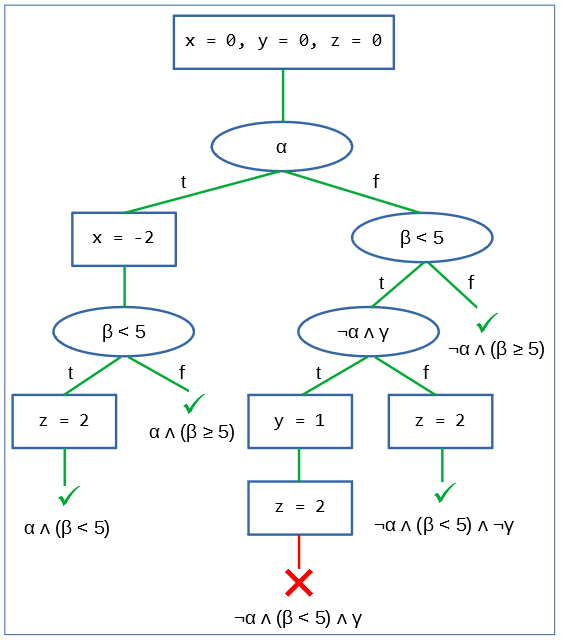
\includegraphics[scale=0.8]{images/sym_tree.png}
    \caption{Drvo simboličkog izvršavanja na kom su prikazane sve putanje koje se razmatraj. Na kraju svake grane je napisan uslov koji mora da važi da bi se došlo do tog lista u drvetu.}
    \label{fig:SymbolicExecTree}
\end{figure}

Simboličko izvršavanje, iako konceptualno moćno, ima par problema:
\begin{itemize}
    \item \emph{eksplozija putanja} - Broj puteva izvršavanja eksponencijalno zavisi od broja uslovnih grananja u kodu. Ukoliko imamo 3 naredbe grananja, broj puteva izvršavanja je $2^3=8$. Štaviše, petlje su još komplikovanije, jer ukoliko imamo u petlji uslov koji zavisi od simboličke vrednosti koja uzima vrednosti iz opsega 32-bitnog celog broja, broj puteva kroz petlju je u tom slučaju $2^31$, a u komplikovanijim slučajevima i beskonačan. Slično važi i za rekuriju.
    \item \emph{ograničenja rešavača} - U nekim slučajevima je moguće osloniti se na \emph{SMT rešavače} \cite{SMT} za nalaženje kontra-primera.
    \item \emph{modelovanje podataka} (engl. \emph{heap modelling}) - Kreiranje simboličkih struktura podataka i pokazivača nije jednostavna.
    \item \emph{modelovanje okruženja} (engl. \emph{environment modelling}) - Nije uvek jednostavno adaptirati mehanizam da radi sa čestim potrebama prilikom dizajna softvera - eksterne biblioteke i sistemski pozivi, specifičnosti sistema i okruženja.
\end{itemize}

Postoji dosta alata i biblioteka koje pružaju simboličko izračunavanje - jedan od najpoznatijih alata za simboličko izračunavanje je \emph{KLEE} \cite{KLEE}, izgrađen nad \emph{LLVM} infrastruktorom \cite{LLVM} i dizajniran za analizu koda pisanog u programskom jeziku C. U nastavku će simboličko izvršavanje biti korišćeno za detekciju razlika u vrednostima promenljivih iz dva AST-a kroz biblioteke za rad sa simboličkim vrednostima u programskom jeziku C\#.

\section{Obrasci za projektovanje}
\label{sec:DesignPatterns}

\emph{Obrasci za projektovanje} (engl. \emph{design patterns} \cite{DesignPatterns}, drugačije nazvani i \emph{projektni šabloni, uzorci}) predstavljaju opšte i ponovno upotrebljivo rešenje čestog problema, obično implementirani kroz koncepte objektno-orijentisanog programiranja. Svaki obrazac za projektovanje ima četiri osnovna elementa:
\begin{itemize}
    \item ime --- ukratko opisuje problem, rešenje i posledice
    \item problem --- opisuje slučaj u kome se obrazac koristi
    \item rešenje --- opisuje elemente dizajna i odnos tih elemenata
    \item posledice --- obuhvataju rezultate i ocene primena obrasca
\end{itemize}

Obrasce za projektovanje je moguće grupisati po situaciji u kojoj se mogu iskoristiti ili načinu na koji rešavaju zadati problem. Stoga je opšte prihvaćena podela na tri grupe:
\begin{itemize}
    \item \emph{gradivni obrasci} (engl. \emph{creational patterns})
    \item \emph{strukturni obrasci} (engl. \emph{structural patterns})
    \item \emph{obrasci ponašanja} (engl. \emph{behavioral patterns})
\end{itemize}

Gradivni obrasci apstrahuju proces pravljenja objekata i važni su kada sistemi više zavise od sastavljanja objekata nego od nasleđivanja. Neki od najvažnijih gradivnih obrazaca su \emph{apstraktna fabrika} (engl. \emph{abstract factory}), \emph{graditelj} (engl. \emph{builder}), \emph{proizvodni metod} (engl. \emph{factory method}), \emph{prototip} (engl. \emph{prototype}) i \emph{unikat} (engl. \emph{singleton}). Strukturni obrasci se bave načinom na koji se klase i objekti sastavljaju u veće strukture. Neki od najvažnijih strukturnih obrazaca su \emph{adapter} (engl. \emph{adapter}), \emph{most} (engl. \emph{bridge}), \emph{sastav} (engl. \emph{composite}), \emph{dekorater} (engl. \emph{decorator}), \emph{fasada} (engl. \emph{facade}), \emph{muva} (engl. \emph{flyweight}) i \emph{proksi} (engl. \emph{proxy}). Obrasci ponašanja se bave načinom na koji se klase i objekti sastavljaju u veće strukture. Neki od najvažnijih strukturnih obrazaca su \emph{lanac odgovornosti} (engl. \emph{chain of responsibility}), \emph{komanda} (engl. \emph{command}), \emph{interpretator} (engl. \emph{interpreter}), \emph{iterator} (engl. \emph{iterator}), \emph{posmatrač} (engl. \emph{observer}), \emph{strategija} (engl. \emph{strategy}) i \emph{posetilac} (engl. \emph{visitor}).

Za potrebe ovog rada, obrasci za projektovanje će se koristiti kao opšte prihvaćeno i programerski intuitivno rešenje određenih problema. Takođe, u kontekstu stabala parsiranja i apstraktnih sintaksičkih stabala opisanih u poglavlju \ref{sec:AST}, obrasci \emph{Posmatrač} i \emph{Posetilac} su od velikog značaja jer pružaju interfejs za obilazak takvih stabala. Ovi obrasci, opisani u narednim odeljcima, se koriste od strane alata korišćenih u ovom radu kao što je ANTLR koji je opisan u odeljku \ref{subsec:ANTLR}. Takođe, s obzirom da su ovi obrasci opšte-prihvaćeno rešenje za pružanje interfejsa obilaska stabala, biće korišćeni i u implementaciji opšte apstrakcije. U nastavku će zbog opisanih razloga biti opisani samo obrasci posmatrač i posetilac, dok zainteresovani čitalac može pročitati više u \cite{DesignPatternsBook}.

\subsection{Obrazac "Posmatrač"}
\label{subsec:DesignPatternsObserver}

Obrazac za projektovanje \emph{Posmatrač} je strukturni obrazac za projektovanje koji se koristi kada je potrebno definisati jedan-ka-više vezu između objekata tako da ukoliko jedan objekat promeni stanje (subjekat) svi zavisni objekti su obavešteni o izmeni i shodno ažurirani. Posmatrač predstavlja \emph{pogled} (engl. \emph{View}) u MVC (engl. \emph{Model-View-Controller}) arhitekturi. Na slici \ref{fig:UMLObserver} se može videti UML dijagram \cite{UML} ovog obrasca. 

\begin{figure}[h!]
\centering
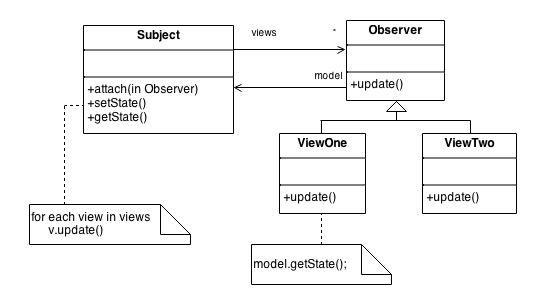
\includegraphics[scale=0.7]{images/observer.jpg}
\caption{UML dijagram obrasca za projektovanje "Posmatrač".} 
\label{fig:UMLObserver}
\end{figure}

Primer upotrebe ovog obrasca može biti aukcija gde je aukcionar subjekat i započinje aukciju, dok učesnici aukcije (objekti) posmatraju aukcionera i reaguju na podizanje cene. Prihvatanje promene cene menja trenutnu cenu i aukcioner oglašava promenu iste, a svi učesnici aukcije dobijaju informaciju da se izmena izvršila. Za potrebe ovog rada, primer upotrebe može biti obilazak stablolike kolekcije (recimo stabla parsiranja) i obaveštavanje o nailasku na čvorove određenih tipova. Te informacije se dalje mogu iskoristiti za izračunavanja nad pomenutom strukturom ili generisanje novih struktura (recimo AST). 

\subsection{Obrazac "Posetilac"}
\label{subsec:DesignPatternsListener}

Obrazac za projektovanje \emph{Posetilac} je strukturni obrazac za projektovanje koji predstavlja operaciju koju je potrebno izvesti nad elementima objektne strukture. Posetilac omogućava definisanje nove operacije bez izmena klasa elemenata nad kojima operiše. Operacija koja će se izvesti zavisi od imena zahteva, tipa posetioca i tipa elementa kog posećuje. Na slici \ref{fig:UMLVisitor} se može videti UML dijagram \cite{UML} ovog obrasca. 

\begin{figure}[h!]
    \centering
    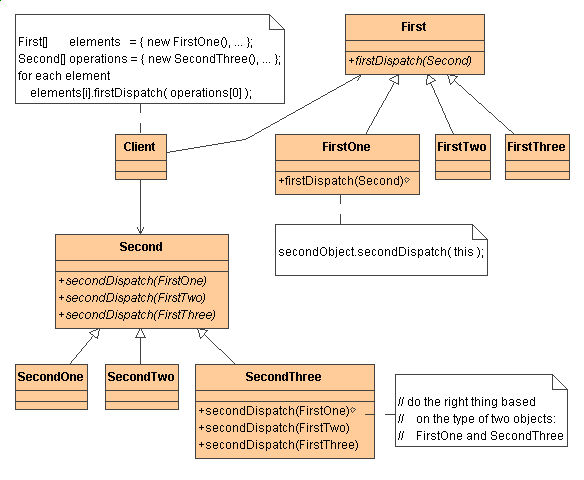
\includegraphics[scale=0.6]{images/visitor.jpg}
    \caption{UML dijagram obrasca za projektovanje "Posetilac".} 
    \label{fig:UMLVisitor}
\end{figure}

Primer upotrebe ovog obrasca može biti operisanje taksi kompanija. Kada osoba pozove taksi kompaniju (prihvatanje posetioca), kompanija šalje vozilo osobi koja je pozvala kompaniju. Nakon ulaska u vozilo (posetilac), mušterija ne kontroliše svoj transport već je to u rukama taksiste (posetioca). Za potrebe ovog rada, primer upotrebe može biti prikupljanje informacija o kolekciji stablolike strukture (recimo stablo parsiranja) i korišćenje istih za neko izračunavanje ili generisanje novih struktura (recimo AST). 

\section{Parsiranje gramatika programskih jezika}
\label{sec:ParsingGrammars}

Pretpostavljajući da imamo gramatiku proizvoljnog programskog jezika, postavlja se pitanje: \emph{Da li je moguće definisati postupak i zatim napraviti program koji će generisati kodove leksera i parsera napisane u određenom programskom jeziku za proizvoljnu gramatiku datu na ulazu?}. Odgovor je potvrdan i postoji veliki broj alata koji se mogu koristiti u ove svrhe, od kojih je navedeno par njih u odeljcima ispod.


\subsection{GNU Bison}
\label{subsec:GNUBison}

\emph{GNU Bison} \cite{GNUBison} je generator parsera i deo GNU projekta \cite{GNUProject}, često referisan samo kao \emph{Bison}. Bison generiše parser na osnovu korisnički definisanih kontekstno slobodnih gramatika \cite{ContextFreeGrammars}, upozoravajući pritom na dvosmislenosti prilikom parsiranja ili nemogućnost primena gramatičkih pravila. Generisani parser je najčešće C a ređe C++ kod, mada se u vreme pisanja ovog rada eksperimentiše sa Java podrškom. Generisani kodovi su u potpunosti prenosivi i ne zahtevaju specifične kompajlere. Bison može da, osim podrazumevanih \emph{LALR(1)} \cite{LALR1} parsera, generiše i kanoničke \emph{LR} \cite{LR}, \emph{IELR(1)} \cite{IELR1} i \emph{GLR} \cite{GLR} parsere.

\subsection{Flex}
\label{subsec:Flex}

\emph{Flex} \cite{Flex} je kreiran kao alternativa \emph{lex}-u \cite{LexYacc}, Flex generiše samo leksere pa se stoga najčešće koristi u kombinaciji sa drugim alatima koji mogu da generišu parsere, kao što je \emph{BYACC}, opisan u nastavku.

\subsection{BYACC}
\label{subsec:BYACC}

\emph{Berkeley YACC}, skraćeno \emph{BYACC} \cite{BYACC}, pisan po ANSI C standardu i otvorenog koda, se smatra od strane mnogih kao \textit{najbolja varijanta YACC-a} \cite{LexYacc}. BYACC dozvoljava tzv. \emph{reentrant} kod - memorija je deljenja između poziva pa je bezbedno konkurentno izvršavanje koda - na način kompatibilan sa Bison-om i to je delom razlog njegove popularnosti.

\subsection{ANTLR}
\label{subsec:ANTLR}
\emph{Another Tool for Language Recognition}, ili kraće \emph{ANTLR} \cite{ANTLR}, je generator \emph{LL(*)} \cite{LLStar} leksera i parsera pisan u programskom jeziku Java sa intuitivnim interfejsom za obilazak stabla parsiranja. Verzija $3$ podržava generisanje parsera u jezicima Ada95, ActionScript, C, C\#, Java, JavaScript, Objective-C, Perl, Python, Ruby, i Standard ML, dok verzija $4$ u vreme pisanja ovog rada samo generiše parsere u narednim jezicima: Java, C\#, C++, JavaScript, Python, Swift i Go.

ANTLR verzije $4$ je izabran u ovom radu zbog svoje jednostavnosti, intuitivnosti i podrške za mnoge moderne programske jezike. Verzija $4$ je izabrana umesto verzije $3$ po preporuci autora, na osnovu eksperimentalne analize brzine i pouzdanosti verzije $4$ u odnosu na verziju $3$. Lekseri i parseri za ulazne gramatike će u implementaciji biti generisani u programskom jeziku C\#.

Parseri generisani koristeći ANTLR koriste novu tehnologiju koja se naziva \emph{Prilagodljiv LL(*)} (engl. \emph{Adaptive LL(*)}) ili \emph{ALL(*)} \cite{ANTLRReference}, dizajniranu od strane Terensa Para, autora ANTLR-a, i Sema Harvela. \emph{ALL(*)} vrši \emph{dinamičku analizu} gramatike u fazi izvršavanja, dok su starije verzije radile analizu pre pokretanja parsera, tzv. \emph{statičku analizu}. Ovaj pristup je takođe efikasniji zbog značajno manjeg prostora ulaznih sekvenci.

Najbolji aspekt ANTLR-a je lakoća definisanja gramatičkih pravila koji opisuju sintaksne konstrukte nalik na aritmetičkim izrazima u programskim jezicima. Primer jednostavnog pravila za definisanje aritmetičkog izraza je dat na slici \ref{fig:ANTLRExpressions}. Pravilo \texttt{exp} je levo rekurzivno jer barem jedna od njegovih alternativnih definicija referiše na baš pravilo \texttt{exp}. ANTLR4 automatski zamenjuje levo rekurzivna pravila u nerekurzivne ekvivalente. Jedini zahtev koji mora biti ispunjen je da levo rekurzivna pravila moraju biti \emph{direktna} - da pravila odmah referišu sama sebe. Pravila ne smeju referisati drugo pravilo sa leve strane definicije takvo da se eventualno kroz rekurziju stigne nazad do pravila od kog se krenulo bez poklapanja sa nekim tokenom.

\begin{figure}[h!]
    \begin{lstlisting}[language={}]
    exp : (exp)
        | exp '*' exp
        | exp '+' exp
        | INT
        ;
    \end{lstlisting}
    \caption{Definicija uprošćenog aritmetičkog izraza u ANTLR4 gramatici.}
    \label{fig:ANTLRExpressions}
\end{figure}


\subsubsection{Preduslovi za pokretanje ANTLR4}
\label{subsubsec:ANTLRInstallation}

Kako bi ANTLR generisao parser u proizvoljnom programskom jeziku, potrebno je instalirati ANTLR i imati \emph{Java Runtime Environment} (skr. \emph{JRE}) instaliran na sistemu i dostupan globalno pokretanjem putem komande \texttt{java}. Instalacija se sastoji od preuzimanja najnovijeg \emph{.jar} fajla
\footnote{Takođe je moguće kompajlirati izvorni kod dostupan na servisu GitHub \url{https://github.com/antlr/antlr4}}, sa zvanične stranice \cite{ANTLR} ili recimo korišćenjem \emph{curl} alata: 
\begin{lstlisting}[language={}]
$ curl -O http://www.antlr.org/download/antlr-4-complete.jar
\end{lstlisting}

Na UNIX sistemima moguće je kreirati alias \texttt{antlr4} ili \emph{shell} skript unutar direktorijuma \texttt{/usr/local/bin} sa imenom \texttt{antlr4} koji će pokrenuti \emph{.jar} fajl na sledeći način (pretpostavljajući da se \emph{.jar} fajl nalazi u direktorijumu \texttt{/usr/local/lib}):
\begin{lstlisting}[language={}]
#!/bin/sh
java -cp "/usr/local/lib/antlr4-complete.jar:$CLASSPATH" org.antlr.v4.Tool $*
\end{lstlisting}

Na Windows sistemima moguće je kreirati \emph{batch} skript sa imenom \texttt{antlr4.bat} koji će pokrenuti ANTLR4, na sledeći način (pretpostavljajući da se \emph{.jar} fajl nalazi u direktorijumu \texttt{C:\textbackslash{}lib}):
\begin{lstlisting}[language={}]
java -cp C:\lib\antlr-4-complete.jar;%CLASSPATH% org.antlr.v4.Tool %*
\end{lstlisting}

Ukoliko su aliasi ili skript fajlovi imenovani kao iznad, moguće je iz komandne linije pojednostavljeno pokretati ANTLR4:  
\begin{lstlisting}[language={}]
$ antlr4
ANTLR Parser Generator Version 4.0
-o ___    specify output directory where all output is generated
-lib ___  specify location of .tokens files
...
\end{lstlisting}

Dodatno, za Unix sisteme \footnote{Za Windows operativni sistem je moguće kreirati \emph{batch} skript po opisu na \url{https://github.com/antlr/antlr4/blob/master/doc/getting-started.md}.}, moguće je kreirati dodatni alias \texttt{grun} (ili alternativno, kreirati \texttt{shell script}) za biblioteku \texttt{TestRig}. Biblioteka TestRig se može koristiti za brzo testiranje parsera - moguće je pokrenuti parser od bilo kog pravila i dobiti izlaz parsera u raznim formatima. TestRig dolazi uz ANTLR \texttt{.jar} fajl i moguće je napraviti prečicu za brzo pokretanje (nalik na ANTLR alias):
\begin{lstlisting}[language={}]
$ alias grun='java -cp "/usr/local/lib/antlr-4-complete.jar:$CLASSPATH" org.antlr.v4.gui.TestRig'
\end{lstlisting}


\subsection{Generisanje parsera koristeći ANTLR4}
\label{subsec:ANTLRParserGeneration}

Prvi korak u izradi aplikacije koja u sebi koristi parsiranje nekog jezika je definisanje gramatike jezika i kreiranje leksera i parsera za isti. U nastavku će biti opisan proces kreiranja interfejsa za parsiranje programa pisanih u pseudo-programskom jeziku (u nastavku \emph{pseudo-jezik}), nalik na pseudokod. Ovako dobijeni interfejs će moći da se koristi u opšte svrhe, za potrebe ovog rada će se koristiti za generisanje AST stabla za program pisan u pseudo-jeziku.

Definišimo gramatiku pseudo-jezika prateći ANTLR pravila za definisanje gramatika. Kao i za svaki drugi programski jezik, treba obezbediti da postoje određeni koncepti koji se pojavljuju u programskim jezicima: \emph{identifikatori}, \emph{izrazi}, \emph{naredbe}, \emph{funkcije} i slično. Za sada se fokusirajmo na naredbe, kao samostalne izvršive jedinice koda. Stoga program možemo smatrati kao niz naredbi. U nekim slučajevima će biti potrebno definisanje kompleksnih naredbi koje se sastoje od više drugih naredbi, i ovakve složene naredbe ćemo zvati \emph{blok} ili \emph{blok naredbi}. Stoga, radi konzistentnosti, program će biti blok naredbi. Kako bismo označili da su naredbe deo bloka naredbi, koristićemo reči \texttt{begin} i \texttt{end}, osim ukoliko je reč o samo jednoj naredbi. Ovakve situacije rešavamo definisanjem \emph{alternativa} u definiciji pravila - više definicija razdvojenih simbolom \texttt{|}. Specijalne reči kao što su \texttt{begin} i \texttt{end} će biti rezervisane reči našeg pseudo-jezika, tzv. \emph{ključne reči}. Na slici \ref{fig:PseudoDef1} se može videti definicija programa \footnote{Drugim rečima, jedan program u pseudo-jeziku je jedinica prevođenja, pa je zato pravilo nazvano \emph{unit}.} i bloka naredbi pseudo-jezika, pri čemu se ključne reči u pravilima navode između apostrofa. ANTLR dozvoljava jednostavne definicije pravila u kojima figuriše promenljiv broj drugih pravila, pri čemu se koriste simboli kao u regularnim izrazima \footnote{U regularnim izrazima, simbol \texttt{a?} označava opciono pojavljivanje simbola \texttt{a}, simbol \texttt{a+} označava jedno ili više pojavljivanja simbola \texttt{a}, a simbol \texttt{a*} označava proizvoljan broj pojavljivanja simbola \texttt{a} - kombinacija simbola \texttt{?} i \texttt{+}.}, što je iskorišćeno za definiciju pravila bloka naredbi. \texttt{NAME} predstavlja ime programa, što je zapravo identifikator. Identifikatore ćemo definisati kasnije, za sada možemo posmatrati identifikator kao nisku karaktera s tim što će postojati restrikcije vezane za to koji karakteri se mogu naći unutar identifikatora ali o tome će biti reči kasnije.

\begin{figure}[h!]
    \begin{lstlisting}[language={}]
    unit
        : 'algorithm' NAME block EOF
        ;
    
    block
        : 'begin' statement+ 'end'
        | statement
        ;
    \end{lstlisting}
    \caption{Definicija jedinice prevođenja i bloka naredbi za pseudo-jezik.}
    \label{fig:PseudoDef1}
\end{figure}

Sledeći korak je definisanje naredbe pseudo-jezika. Slično kao i u drugim programskim jezicima, potrebno je podržati koncept deklaracije promenljive, dodele vrednosti izraza promenljivoj, naredbe kontrole toka - grananje i petlje. Na slici \ref{fig:PseudoDef2} je definisano šta se sve smatra jednom naredbom. Naredbe mogu biti i prazne, što je označeno ključnom rečju \texttt{pass}. Iz definicije naredbe sa slike se jasno vidi šta sve može biti naredba (prateći redosled alternativa pravila):
\begin{itemize}
    \item deklaracija
    \item dodela
    \item poziv funkcije (označen kao \texttt{cexp}, skraćeno od \emph{function call expression}) \footnote{Funkcije mogu vratiti vrednosti pa se stoga njihovi pozivi mogu naći u izrazima - dakle poziv funkcije je validan izraz (stoga \texttt{expression} u imenu \texttt{function call expression}). Naravno, ta vrednost se može ignorisati ili pak sama funkcija može biti takva da nema povratnu vrednost već je samo neophodno izvršiti je zbog sporednih efekata.}
    \item vraćanje vrednosti izraza (ključna vrednost \texttt{return}) iz funkcije
    \item prekidanje izvršavanja davanjem poruke o grešci
    \item naredba grananja
    \item \emph{while} petlja
    \item \emph{repeat-until} petlja
    \item inkrementiranje/dekrementiranje vrednosti promenljive
\end{itemize}
    
\begin{figure}[h!]
    \begin{lstlisting}[language={}]
    statement
        : 'pass'
        | declaration
        | assignment
        | cexp
        | 'return' exp
        | 'error' STRING
        | 'if' exp 'then' block ('else' block)? 
        | 'while' exp 'do' block 
        | 'repeat' block 'until' exp
        | ('increment' | 'decrement') var	
        ;
    \end{lstlisting}
    \caption{Definicija naredbe za pseudo-jezik.}
    \label{fig:PseudoDef2}
\end{figure}

Deklaracija, prikazana na slici \ref{fig:PseudoDef3}, uvodi pojavljivanje simbola datog preko identifikatora \texttt{NAME} kao oznaku za promenljivu, funkciju ili proceduru - funkciju bez povratne vrednosti. Svaka promenljiva mora biti određenog tipa, što se postiže pravilom \texttt{type}. Promenljivoj se, opciono, može pridružiti početna vrednost, drugim rečima promenljiva se može \emph{inicijalizovati} tako da joj se pridruži vrednost nekog izraza. Procedure i funkcije imaju opcione parametre, vrednosti izraza koje im se prosleđuju kasnije u pozivu kao argumenti. Lista parametara, takođe prikazana na slici \ref{fig:PseudoDef3}, se navodi kao lista proizvoljno mnogo parova \texttt{NAME : type}, što se vidi iz definicije pravila \texttt{parlist}.

\begin{figure}[h!]
    \begin{lstlisting}[language={}]
    declaration
        : 'declare' type NAME ('=' exp)? 
        | 'procedure' NAME '(' parlist? ')' block 
        | 'function' NAME '(' parlist? ')' 'returning' type block 
        ;

    parlist
        : NAME ':' type (',' NAME ':' type)*
        ;
    \end{lstlisting}
    \caption{Definicija deklaracije za pseudo-jezik.}
    \label{fig:PseudoDef3}
\end{figure}

Identifikatori su niske karaktera koje predstavljaju ime koje odgovara određenoj memorijskoj adresi. Identifikatori se koriste umesto sirovih vrednosti adresa kako bi kod bio čitljiviji i lakši za pisanje - na nivou asemblera se većinom koriste adrese ili automatski generisane oznake. Na slici \ref{fig:PseudoDef4} se može videti definicija identifikatora. Identifikator se sastoji od slova, cifara i simbola \texttt{\_}, s tim što ne sme početi cifrom. Ovo je konvencija koju prati dosta jezika, uključujući programski jezik C. Primetimo da je identifikator nešto što bi lekser trebalo da prepozna tokom tokenizacije. Međutim, kada definišemo gramatiku od koje će ANTLR praviti lekser i parser, možemo i tokene definisati preko gramatičih pravila dajući regularni izraz za njihovo poklapanje. Listovi stabla parsiranja su uvek tokeni, drugim rečima se nazivaju i \emph{terminalni simboli}. Tokeni se, naravno, mogu naći bilo gde u stablu parsiranja.

\begin{figure}[h!]
    \begin{lstlisting}[language={}]
    NAME
        : [a-zA-Z_][a-zA-Z_0-9]*
        ;
    \end{lstlisting}
    \caption{Definicija identifikatora za pseudo-jezik.}
    \label{fig:PseudoDef4}
\end{figure}

Pošto želimo da pseudo-jezik bude strogo tipiziran, potreban je koncept tipa (što smo videli u deklaracijama), čija je definicija data na slici \ref{fig:PseudoDef5}. Tip može biti \emph{primitivan} (drugim rečima \emph{prost}) ili \emph{složen}. Primitivni tipovi su podržani u samoj sintaksi jezika - u našem slučaju brojevi i niske. Brojevi mogu biti celi ili realni. U složene tipove spadaju korisnički definisani tipovi (sa imenom \texttt{NAME}, u četvrtoj alternativi pravila \texttt{typename} sa slike \ref{fig:PseudoDef5}) i kolekcije. Od kolekcija su podržani nizovi, liste i skupovi. Prilikom definicije kolekcije mora se navesti tip elemenata kolekcije i taj tip mora biti uniforman - isti za sve elemente kolekcije. 

\begin{figure}[h!]
    \begin{lstlisting}[language={}]
    type 
        : typename 'array'?
        | typename 'list'?
        | typename 'set'?
        ;

    typename 
        : 'integer' 
        | 'real' 
        | 'string' 
        | NAME 
        ;
    \end{lstlisting}
    \caption{Definicija tipa podataka za pseudo-jezik.}
    \label{fig:PseudoDef5}
\end{figure}

Izrazi, iako se definišu rekurzivno, se mogu posmatrati kao kombinacija promenljivih, operatora i poziva funkcija sa odlikom da se mogu \emph{evaluirati}, tj. moguće je izračunati njegovu vrednost. Iz definicije pravila \texttt{exp} na slici \ref{fig:PseudoDef6}, mogu se uočiti tipovi izraza, pri čemu nije vođeno računa o matematičkom prioritetu operatora, radi jednostavnosti. Izraz može biti \emph{literal}, koji predstavlja konstantu, bilo brojevnu, logičku ili nisku karaktera. Promenljive, definisane pravilom \texttt{var} su takođe izrazi, jer se trenutna vrednost promenljive posmatra kao vrednosti izraza. Primetimo da promenljiva može biti kolekcijskog tipa, u kom slučaju se navodi redni broj elementa nakon identifikatora promenljive - taj redni broj može biti rezultat evaluacije drugog izraza, ali ne bilo kakvog, stoga se u pravilu \texttt{iexp} definiše šta sve može biti korišćeno da se indeksira element kolekcije. Izrazima se može dati prioritet pomoću zagrada, što se vidi u trećoj alternativi pravila \texttt{exp}. U naredne tri alternative su opisani tipovi izraza: aritmetički, relacioni i logički. Aritmetički izrazi su vezani aritmetičkim operatorima definisanim preko pravila \texttt{aop}, slično važi i za ostala dva tipa. Svi tipovi izraza navedeni iznad su binarni, što znači da operatori zahtevaju dva argumenta. Postoje i unarni izrazi, od kojih su podržane promena znaka i logička negacija, što se vidi iz pravila \texttt{uop}.

\begin{figure}[h!]
    \begin{lstlisting}[language={}]
    exp
        : literal 
        | var
        | '(' exp ')'
        | exp aop exp
        | exp rop exp
        | exp lop exp
        | uop exp
        | cexp
        ;

    var 
        : NAME ('[' iexp ']')?
        ;
    
    iexp 
        : literal
        | var
        | aexp
        ;

    cexp
        : 'call' NAME '(' explist? ')'
        ;

    explist
        : exp (',' exp)*
        ;

    aop : '+' | '-' | '*' | '/' | 'div' | 'mod' ;
    rop : '>' | '>=' | '<' | '<=' | '==' | '=/=' ;
    lop : 'and' | 'or' ;
    uop : '-' | 'not' ;
    \end{lstlisting}
    \caption{Definicija izraza za pseudo-jezik.}
    \label{fig:PseudoDef6}
\end{figure}

Definicija literala je prikazana na slici \ref{fig:PseudoDef7}. Literali mogu bili istinitosne konstante \texttt{True} i \texttt{False}, brojevne konstante ili niske karaktera. Brojevne konstante mogu bili celobrojni ili realni dekadni brojevi. Realne konstatne je moguće definisati u fiksnom ili pokretnom zarezu. Niske se mogu definisati između navodnika ili apostrofa. Pritom, kao i u modernim programskim jezicima, moguće je navesti sekvence koje predstavljaju specijalne karaktere kao što su novi red, tabulator itd. Oznaka \texttt{fragment} označava optimizaciju, naime nije potrebno da postoji na primer pravilo \texttt{Digit}, već samo dajemo simbol za regularni izraz koji će se koristiti u više drugih pravila i poklapati jednu dekadnu cifru.

\begin{figure}[h!]
    \begin{lstlisting}[language={}]
    literal : 'True' | 'False' | INT | FLOAT | STRING ;

    STRING
        : '"' ( EscapeSequence | ~('\\'|'"') )* '"' 
        ;

    fragment
    EscapeSequence
        : '\\' [abfnrtvz"'\\]
        | '\\' '\r'? '\n'
        ;

    INT
        : Digit+
        ;

    FLOAT
        : Digit+ '.' Digit* ExponentPart?
        | '.' Digit+ ExponentPart?
        | Digit+ ExponentPart
        ;

    fragment
    ExponentPart
        : [eE] [+-]? Digit+
        ;

    fragment
    Digit
        : [0-9]
        ;
    \end{lstlisting}
    \caption{Definicija konstanti za pseudo-jezik.}
    \label{fig:PseudoDef7}
\end{figure}

Poslednje što treba definisati je sve ono što lekser treba da preskoči tokom prolaska kroz izvorni kod programa. To su beline (nevidljivi karakteri kao što su razmaci, tabulatori i novi redovi) i komentari. Definicije ovih pravila se mogu videti na slici \ref{fig:PseudoDef8}. Vidimo da se u njima koristi posebna oznaka \texttt{-> skip}, koja predstavlja instrukcije lekseru da preskoči sve ono što ovo pravilo poklopi. Komentari su u stilu kao u programskom jeziku C (ali naravno, isti stil se koristi i u mnogim jezicima) i mogu biti jednolinijski ili višelinijski. Beline koje treba preskočiti su definisane u pravilu \texttt{WS}, skraćeno od \emph{whitespace}, što u prevodu sa engleskog znači \emph{beli prostor, belina}.

\begin{figure}[h!]
    \begin{lstlisting}[language={}]
    BlockComment
        :   '/*' .*? '*/'  -> skip
        ;
    LineComment
        :   '//' ~[\r\n]*  -> skip
        ;
    WS  
        : [ \t\u000C\r\n]+ -> skip
        ;
    \end{lstlisting}
    \caption{Definicija komentara i belina za pseudo-jezik.}
    \label{fig:PseudoDef8}
\end{figure}

\begin{figure}[h!]
    \begin{lstlisting}[language={}]
    grammar Pseudo;
    \end{lstlisting}
    \caption{Definicija imena gramatike za pseudo-jezik.}
    \label{fig:PseudoDef9}
\end{figure}

Ovako definisanu gramatiku možemo sačuvati u fajl sa imenom \texttt{Pseudo.g4}, potrebno je samo navesti ime gramatike na početku fajla, kao na slici \ref{fig:PseudoDef9}. Naredni korak je kreiranje leksera i parsera koristeći ANTLR4, predpostavljajući da je instaliran na način opisan u \ref{subsec:ANTLRInstallation}. Pokretanjem ANTLR-a generišemo lekser i parser za gramatiku pseudo-jezika:
\begin{lstlisting}[language={}]
$ antlr4 Pseudo.g4
\end{lstlisting}

ANTLR4 će generisati lekser i parser podrazumevano napisane u programskom jeziku Java. Ukoliko želimo to da promenimo, možemo koristiti opciju \texttt{-Dlanguage=...}. Kako bismo testirali generisani lekser i parser, možemo koristiti ANTLR TestRig da vizualno prikažemo stablo parsiranja, s tim što moramo prvo kompajlirati generisane Java kodove. TestRig pozivamo navođenjem ime gramatike (koje se poklapa sa imenom leksera i parsera) i imenom pravila od koga će parser krenuti. Opcija \texttt{-gui} pokreće vizualni prikaz stabla parsiranja pokazan na slici \ref{fig:PseudoTreeGui} (vizualni prikaz je moguće preskočiti i samo ispisati stablo u LISP formi koristeći opciju \texttt{-tree}), mada je moguće i ispisati samo tokene koristeći opciju \texttt{-tokens}. Ulaz se prosleđuje programu dok se ne naiđe na simbol \texttt{EOF}, ili alternativno se može preneti ulaz putem UNIX pipeline-a (na slici \ref{fig:PseudoTreeGui} se može videti izlaz koji se dobija korišćenjem opcije \texttt{-gui}):
\begin{lstlisting}[language={}]
$ javac *.java
$ echo "declare integer x = 5" | grun Pseudo declaration -tokens
[@0,0:6='declare',<'declare'>,1:0]
[@1,8:14='integer',<'integer'>,1:8]
[@2,16:16='x',<NAME>,1:16]
[@3,18:18='=',<'='>,1:18]
[@4,20:20='5',<INT>,1:20]
[@5,22:21='<EOF>',<EOF>,2:0]
$ echo "declare integer x = 5" | grun Pseudo declaration -tree
(declaration declare (type (typename integer)) x = (exp (literal 5)))
$ echo "declare integer x = 5" | grun Pseudo declaration -gui
\end{lstlisting}    

\begin{figure}[h!]
    \centering
        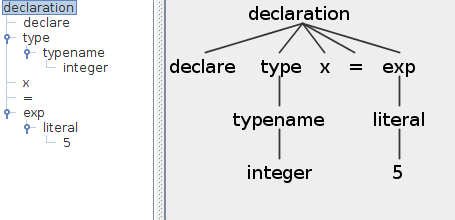
\includegraphics[scale=0.8]{images/pseudo_parse_tree.png}
    \caption{Grafički prikaz stabla parsiranja koje generiše parser kreiran od strane alata ANTLR4 TestRig za kod pisan u pseudo-jeziku.}
    \label{fig:PseudoTreeGui}
\end{figure}


\subsection{Obilazak stabla parsiranja}
\label{subsec:ANTLRParserIntegration}

ANTLR, osim leksera i parsera za datu gramatiku, može da kreira interfejse i bazne klase koji prate obrasce za projektovanje \emph{posetilac} (engl. \emph{visitor}) i osluškivač (engl. \emph{listener}, varijanta obrasca \emph{posmatrač} engl. \emph{observer}) opisane u \ref{sec:DesignPatterns}. Tako kreirani interfejsi i klase imaju metodi za obilazak stabla parsiranja. ANTLR podrazumevano generiše interfejs osluškivača (slika \ref{fig:ANTLRListener}) kao i baznu klasu koja implementira generisani interfejs tako što su sve implementirane metodi prazne. Stoga, ukoliko korisnik želi da definiše operaciju samo u slučaju da se prilikom obilaska stabla parsiranja naiđe na samo jedan tip čvora, nije potrebno implementirati ceo interfejs osluškivača, već je moguće naslediti baznu klasu i predefinisati samo jedan metod. ANTLR može da generiše i posetilac (slika \ref{fig:ANTLRVisitor}), ukoliko se navede odgovarajuća opcija \texttt{-visitor} prilikom pokretanja. Slično, ukoliko nije potrebno generisati osluškivač, može se koristiti opcija \texttt{-no-listener} kako se ne bi generisao osluškivač.

\begin{figure}[h!]
\begin{lstlisting}
public interface IPseudoListener : IParseTreeListener
{
    void EnterUnit([NotNull] PseudoParser.UnitContext context);
    void ExitUnit([NotNull] PseudoParser.UnitContext context);
    void EnterBlock([NotNull] PseudoParser.BlockContext context);
    void ExitBlock([NotNull] PseudoParser.BlockContext context);
    void EnterStatement([NotNull] PseudoParser.StatementContext context);
    void ExitStatement([NotNull] PseudoParser.StatementContext context);
    
    ...
}
\end{lstlisting}
\caption{Delimični prikaz interfejsa osluškivača generisanog od strane ANTLR4 za pseudo-jezik definisan u prethodnom odeljku (C\#).}
\label{fig:ANTLRListener}
\end{figure}

Sa slike \ref{fig:ANTLRListener} se vidi da je moguće definisati metodi koje će se pozivati prilikom ulaska ali i prilikom izlaska iz čvora određenog tipa prilikom obilaska stabla parsiranja. Pritom, važno je kako se stablo obilazi. U slučaju ANTLR, to je pretraga u dubinu (engl. \emph{depth-first search, DFS}) \footnote{DFS je obilazak stabla takav da se obilazak duž grane stabla nastavlja sve dok je moguće ići dublje, a ako to nije moguće vratiti se unazad i obići druge grane.}, stoga će se metod \texttt{Exit} za proizvoljni čvor pozvati tek kad se obiđu sva deca tog čvora - dakle nakon poziva njihovih \texttt{Enter} i \texttt{Exit} metoda. Pošto se DFS obično implementira putem LIFO \footnote{\emph{Last In, First Out} struktura podataka je apstraktna struktura podataka sa operacijama ubacivanja i izbacivanja elemenata, pri čemu je element koji se izbacuje onaj koji je poslednji ubačen. Primer LIFO strukture je držač za CD-ove - ne mogu se ukloniti CD-ovi ispod CD-a na vrhu (poslednji ubačen) a da se ne ukloni isti. U slučaju opisanom iznad, implementacija LIFO strukture se naziva stek \emph{stack}.} strukture, može se reći da se \texttt{Enter} metod poziva onog trenutka kad se čvor ubaci u strukturu, a \texttt{Exit} metod onda kada se čvor ukloni iz strukture.

\begin{figure}[h!]
\begin{lstlisting}
public interface IPseudoVisitor<Result> : IParseTreeVisitor<Result>
{
    Result VisitUnit([NotNull] PseudoParser.UnitContext context);
    Result VisitBlock([NotNull] PseudoParser.BlockContext context);
    Result VisitStatement([NotNull] PseudoParser.StatementContext context);
    Result VisitDeclaration([NotNull] PseudoParser.DeclarationContext context);
    
    ...
}
\end{lstlisting}
\caption{Delimični prikaz interfejsa posetioca generisanog od strane ANTLR4 za pseudo-jezik definisan u prethodnom odeljku (C\#).}
\label{fig:ANTLRVisitor}
\end{figure}

Za razliku od osluškivača, posetilac je prirodnije koristiti ukoliko je potrebno izvršiti neko izračunavanje nad strukturom koja se obilazi. Interfejs posetioca (slika \ref{fig:ANTLRVisitor}) je šablonski, i metodi imaju povratnu vrednost šablonskog tipa za razliku od metoda osluškivača i, u odnosu na osluškivač, nema para metoda za svaki čvor već samo jedan metod. Dodatna razlika, ali i najveća, je ta što se metodi posetioca ne pozivaju automatski. Stoga je na programeru da nastavi obilazak i da odluči u koje čvorove želi da se spusti. Jasno je da i osluškivač i posetilac imaju svoje primene - ukoliko je potrebno obići stablo parsiranja i dovući neke informacije može se iskoristiti osluškivač jer onda ne moramo brinuti o obilasku. S druge strane, ukoliko je potrebno izračunati neku vrednost prirodno je iskoristiti rekurziju i iskoristiti posetilac - rekurzivni pozivi prilikom obilaska nam idu u prilog jer koristimo povratne vrednosti tih metoda da gradimo rezultat od listova ka korenu stabla parsiranja. U nastavku će se koristiti posetilac zbog kontrole obilaska ali i činjenice da se stablo parsiranja obilazi sa ciljem da se izgradi AST, koji je takođe rekurzivna struktura i gradi se inkrementalno kroz rekurziju.

Bilo da se koristi osluškivač ili posetilac, potrebno je nekako proslediti informacije o samom čvoru na koji se naišlo tokom obilaska stabla parsiranja. Te informacije se metodima osluškivača i posetioca prosleđuju putem potklasa apstrakne klase konteksta pravila \texttt{ParserRuleContext} - u primeru iznad \texttt{UnitContext}, \texttt{BlockContext} itd. Svaki kontekst pravila po imenu odgovara pravilima definisanim u gramatici i sadrži informacije bitne za trenutni čvor u stablu parsiranja koji odgovara tipu konteksta. Takođe, u svakom kontekstu su prisutne i metodi čija imena odgovaraju pravilima koja se javljaju u definiciji samog pravila koje odgovara kontekstu. Tako da, za \texttt{BlockContext}, imajući u vidu definiciju sa slike \ref{fig:PseudoDef1}, pošto se u definiciji osim tokena koristi i pravilo \texttt{statement}, u okviru \texttt{BlockContext} klase biće implementiran i metod \texttt{statement()} koji vraća kontekst pravila u ovom slučaju tipa \texttt{StatementContext[]} jer u prvoj alternativi stoji \texttt{statement+} - dakle možemo imati više \texttt{statement} poklapanja. Sa ovim u vidu, moguće je odrediti kako će se obilazak nastaviti (u slučaju posetioca) ili dovući informacije o delovima definicije pravila. Ukoliko pravilo ima više alternativa, metodi koje vraćaju kontekst pravila koje figuriše u alternativi koja nije korišćena za poklapanje pravila će vratiti \texttt{null}. Pošto se \texttt{statement()} pravilo javlja u obe alternative pravila \texttt{block} (i nije opciono), možemo biti sigurni da povratna vrednost \texttt{statement()} metoda nikada neće biti \texttt{null}.

U poglavlju \ref{chp:MyAST} će se koristiti posetilac za obilazak stabla parsiranja i kreiranje AST apstrakcije od istog. Pritom, koristiće se implementacija posetioca u programskom jeziku C\#. Pre toga, potrebno je objasniti pojam \emph{simboličke promenljive} s obzirom da će se ti koncepti koristiti u samoj analizi AST-ova.

\section{Programske paradigme i gramatičke razlike programskih jezika}
\label{sec:Paradigms}

Iako se u suštini svode na mašinski jezik ili asembler, viši programski jezici mogu imati velike razlike međusobno - kako u načinu pisanja koda, tako i u efikasnosti izvršavanja. Način, ili stil programiranja se naziva \emph{programska paradigma} \cite{ProgrammingParadigms}. Može se pokazati da sve što je rešivo putem jedne, može i da se reši i putem ostalih; međutim neki problemi se prirodnije rešavaju koristeći specifične paradigme. Neke poznatije programske paradigme su navedene u nastavku zajedno sa njihovim odlikama i primerima upotrebe.

\subsection{Imperativna paradigma}
\label{subsec:ParadigmImperative}

\emph{Imperativna paradigma} pretpostavlja da se promene u trenutnom stanju izvršavanja mogu sačuvati kroz promenljive. Izračunvanja se vrše kroz niz koraka, u svakom koraku se te promenljive referišu ili se menjaju njihove trenutne vrednosti. Raspored koraka je bitan, jer svaki korak može imati različite posledice s obzirom na trenutne vrednosti promenljivih na početku tog koraka. Primer koda pisanog po imperativnoj paradigmi se može videti na slici \ref{fig:ParadigmImperative}.

\begin{figure}[h!]
\begin{lstlisting}
    result = []
    i = 0
start:
    numPeople = length(people)
    if i >= numPeople goto finished
    p = people[i]
    nameLength = length(p.name)
    if nameLength <= 5 goto nextOne
    upperName = toUpper(p.name)
    addToList(result, upperName)
nextOne:
    i = i + 1
    goto start
finished:
    return sort(result)
\end{lstlisting}
\caption{Primer koda pisanog po imperativnoj paradigmi.}
\label{fig:ParadigmImperative}
\end{figure}

Imperativni programski jezici najčešće prate ovu paradigmu više nego bilo koju drugu iz par razloga. Prvi je taj što imperativna paradigma najbliže oslikava samu mašinu na kojoj se program izvršava, pa je programer mnogo "bliži" istoj. Posledica ovog pristupa, a to je i drugi razlog za popularnost imperativne paradigme, je omogućila da je ova paradigma bila najefikasnija zbog ograničenja u hardveru. Danas, zbog mnogo bržeg razvoja i mnogo jačih računara, efikasnost se sve manje i manje uzima u obzir.

Naravno, imperativna paradigma ima i svoje nedostatke. Naime, najveći problem je razumevanje i verifikovanje semantike programa zbog postojanja sporednih efekata \footnote{Sporedni efekti (promena stanja mašine) ne poštuju \emph{referencijalnu transparentnost} koja se definiše na sledeći način: \emph{Ako važi $P(x)$ i $x = y$ u nekom trenutku, onda $P(x) = P(y)$ važi tokom čitavog vremena izvršavanja programa}.}. Stoga je i pronalaženje grešaka u kodovima koji prate imperativnu paradigmu znatno komplikovanije. Apstrakcija je takođe više ograničena u imperativnoj nego u ostalim paradigmama. Na kraju, redosled izvršavanja je vrlo bitan, što neke probleme čini težim ukoliko se pokušaju rešiti pomoću imperativne paradigme.

\subsection{Strukturna paradigma}
\label{subsec:ParadigmImperativeStructural}

\emph{Strukturna paradigma} je vrsta imperativne paradigme gde se kontrola toka vrši putem ugnježdenih petlji, uslovnih grananja i podrutina. Promenljive su obično lokalne za blok u kome su definisane, što određuje i njihov životni vek i vidljivost. Primer koda pisanog po imperativnoj paradigmi se može videti na slici \ref{fig:ParadigmStructural}. Najpopularniji derivat strukturne paradigme je \emph{proceduralna paradigma}, bazirana na konceptu poziva \emph{procedure} - podrutine ili funkcije koja sadrži seriju koraka koje je potrebno izvršiti redom.

\begin{figure}[h!]
\begin{lstlisting}
result = [];
for i = 0; i < length(people); i++ {
    p = people[i];
    if length(p.name)) > 5 {
        addToList(result, toUpper(p.name));
    }
}
return sort(result);
\end{lstlisting}
\caption{Primer koda pisanog po strukturnoj paradigmi.}
\label{fig:ParadigmStructural}
\end{figure}


\subsection{Logička paradigma}
\label{subsec:ParadigmLogical}

\emph{Logička paradigma} koristi deklarativni pristup rešavanju problema. Umesto zadavanja instrukcije koje treba da dovedu do rezultata, opisuje se sam rezultat kroz činjenice - skup logičkih pretpostavki. Taj opis se zatim prevodi u upit koji se dalje koristi. Uloga računara je održvanje i logička dedukcija. Logička paradigma se deli u tri sekcije:
\begin{itemize}
    \item niz deklaracija i definicija koje opisuju problem iz nekog domena,
    \item relevantne činjenice i
    \item relevantni ciljevi u formi upita.
\end{itemize}

Bilo koji rezultat dedukcije rešenja upita predstavlja rezultat izvršavanja. Deklaracije i definicije se konstruišu iz relacija, npr. $X \in Y$ ili $X \in [a,b]$. Prednost ovog pristupa je mala količina programiranja, pošto dedukcioni sistem traži rešenje problema. Takođe, verifikovanje validnosti je stoga trivijalno. Primer koda pisanog po logičkoj paradigmi se može videti na slici \ref{fig:ParadigmLogical}.

\begin{figure}[h!]
\begin{lstlisting}
domains
    being = symbol 
predicates
    animal(being)       % sve životinje su bića
    dog(being)          % svi psi su bića
    die(being)          % svi bića umiru 
clauses
    animal(X) :- dog(X) % svi psi su životinje
    dog(fido).          % fido je pas
    die(X) :- animal(X) % sve životinje umiru 
\end{lstlisting}
\caption{Primer koda pisanog po logičkoj paradigmi.}
\label{fig:ParadigmLogical}
\end{figure}


\subsection{Funkcionalna paradigma}
\label{subsec:ParadigmFunctional}

\emph{Funkcionalna paradigma} posmatra sve potprograme kao funkcije u matematičkom smislu - uzimaju argumente i vraćaju jedinstven rezultat. Povratna vrednost zavisi isključivo od argumenata, što znači da je nebitan trenutak u kom je funkcija pozvana. Izračunvanja se vrše primenom aplikacije funkcija, kompozicijom funkcija i redukcijom. Primer koda pisanog po logičkoj paradigmi se može videti na slici \ref{fig:ParadigmFunctional}.

\begin{figure}[h!]
\begin{lstlisting}
people 
    |> map    (extract_name . to_upper) 
    |> filter (\name -> length name > 5) 
    |> sort
    |> take 5
    |> join ", "
\end{lstlisting}
\caption{Primer koda pisanog po funkcionalnoj paradigmi.}
\label{fig:ParadigmFunctional}
\end{figure}
    
Funkcionalni programski jezici se baziraju na funkcionalnoj paradigmi. Takvi jezici dozvoljavaju tretiranje funkcija kao \emph{građana prvog reda} - mogu biti tretirane kao podaci pa se mogu proslediti drugim funkcijama ili vratiti kao rezultat izračunavanja drugih funkcija. Prednosti funkcionalnih jezika su visok nivo apstrakcije, što prevazilazi mnogo detalja programiranja i stoga eliminiše pojavu velikog broja grešaka, nezavisnost od redosleda izračunavanja, što omogućava paralelizam, i formalnu matematičku verifikaciju. Mane su potencijalna manja efikasnost, što danas predstavlja manji problem, kao i teškoća implementacije specifične sekvencijalne aktivnosti ili potreba za stanjem, što bi se lako implementiralo imperativno ili preko OO paradigme.


\subsection{Objektno-orijentisana paradigma}
\label{subsec:ParadigmOOP}

\emph{Objektno-orijentisana paradigma} (kraće \emph{OOP}) je paradigma u kojoj se objekti stvarnog sveta posmatraju kao zasebni entiteti koji imaju sopstveno stanje koje se modifikuje samo pomoću procedura ugrađenih u same objekte - tzv. \emph{metode}. Posledica zasebnog operisanja objekata omogućava njihovu enkapsulaciju u module koji sadrže lokalnu sredinu i metode. Komunikacija sa objektom se vrši prosleđivanjem poruka. Objekti su organizovani u klase, od kojih nasleđuju metode i ekvivalentne promenljive. OOP omogućava ponovnu iskorišćenost koda i ekstenzibilnost koda. Primer koda po strukturnoj paradigmi je dat na slici \ref{fig:ParadigmOOP}. 

\begin{figure}[h!]
\begin{lstlisting}
abstract class Employee
{
    private String name;

    Employee(String name) {
        this.name = name;
    }

    abstract void work();
};

class WageEmployee extends Employee
{
    private double wage;
    private double hours;

    WageEmployee(String name) {
        super(name);
        this.name = name;
    }

    void work() {
        wage += 200;
        hours += 8;
    }
};

var bill = new WageEmployee("Bill Gates");
bill.work();
\end{lstlisting}
\caption{Primer koda pisanog po OO paradigmi u programskom jeziku Java.}
\label{fig:ParadigmOOP}
\end{figure}

Nova klasa ($A$) može \emph{naslediti} ili \emph{konkretizovati} drugu klasu ($B$). $B$ se zove \emph{bazna klasa} ili \emph{natklasa}, dok se $A$ naziva \emph{izvedena klasa} ili \emph{potklasa}. Izvedenna klasa nasleđuje sve odlike bazne klase - strukturu i ponašanje - postaje specijalizacija bazne klase dok bazna klasa postaje generalizacija svoje potklase. Osim nasleđenih osobina, potklasa može imati dodatna stanja (instancne promenljive) ili dodatna ponašanja (metode). Dozvoljeno je i predefinisanje ponašanja bazne klase. Mehanizam nasleđivanja je dozvoljen i ukoliko nije dozvoljen pristup izvornom kodu bazne klase.

Idealno, stanju objekta može da pristupi i modifikuje samo pomoću metoda tog objekta. Većina OO jezika dozvoljava direktnu manipulaciju stanja ali taj pristup nije preporučen. Kako bi se enkapsulacija i skrivanje informacija kao najveće prednosti OO paradigme mogle iskoristiti, interfejs klase (kako se pristupa objektima) bi trebalo da bude odvojen od implementacije klase (izvornog koda metoda klasa).


\subsection{Skript paradigma i njen odnos sa proceduralnom paradigmom}
\label{subsec:Languages}

Čak i unutar jedne paradigme kao što je proceduralna paradigma, mogu se naći veoma velike varijacije u izgledu koda pisanog u različitim programskim jezicima koji prate proceduralnu paradigmu. Kako hardver postaje moćniji, više se ceni vreme koje programer provede u procesu pisanja koda nego koliko je taj kod efikasan. Štaviše, u nekim slučajevima je dobitak u efikasnosti veoma mali u poređenju sa vremenom koje je potrebno utrošiti da bi se ta efikasnost postigla. Ukoliko se program pokreće veoma retko, možda nije ni bitno da li se on izvršava sekundu sporije od efikasnog programa, ako je za njegovo pisanje utrošeno znatno manje vremena. Ovo je pristup koji prate \emph{skript} jezici kao što su \texttt{Python, Perl, bash} itd. Iako proceduralni, oni se razlikuju od klasičnih predstavnika proceduralne paradigme i njihove razlike su vremenom postale tolike da nije neuobičajeno da se skript jezici svrstaju u zasebnu, \emph{skript paradigmu}. Stoga će se u nastavku, pod terminom \emph{proceduralni jezik} smatrati tradicionalni proceduralni jezik, ukoliko nije naznačeno drugačije. Na slici \ref{fig:LanguagesDiff} se mogu uočiti navedene razlike.

\begin{figure}[h!]
\begin{lstlisting}
int main() {
    int k = 0;
    for (int i = 0; i < 1000000; i++)
        k++;
    return 0;
}
\end{lstlisting}
\begin{lstlisting}[language={}]
$ time: 0.03s user 0.00s system 70% cpu 0.044 total
\end{lstlisting}
\begin{lstlisting}
k = 0
for i in range(1000000):
    k += 1
\end{lstlisting}
\begin{lstlisting}[language={}]
$ time: 0.16s user 0.03s system 93% cpu 0.200 total
\end{lstlisting}
\caption{Primer koda pisanog po tradicionalnoj proceduralnoj paradigmi (gore, \texttt{C}) i po modernoj skript paradigmi (gore, \texttt{Python 3}) kao i odgovarajuća vremena izvršavanja dobijena komandom \texttt{time}.}
\label{fig:LanguagesDiff}
\end{figure}

Promenljive predstavljaju jedan od osnovnih koncepata na kojem se zasnivaju i proceduralni i skript jezici. Promenljivu odlikuje, između ostalog, i njen \emph{tip} koji određuje količinu memorije potrebnu za njeno skladištenje. Proceduralni programski jezici zahtevaju definisanje tipa promenljive i obično su i \emph{statički}, što znači da promenljive ne mogu menjati svoj tip tokom izvršavanja programa. Skript jezici žrtvuju strogu tipiziranost kako bi proces pisanja koda bio brži. Stoga su oni obično \emph{dinamički} - promenljive mogu menjati tip tokom izvršavanja programa. Pošto promenljive mogu menjati svoj tip, definisanje tipa prilikom uvođenja imena promenljive postaje redundantno jer prevodilac može to sam da zaključi. Stoga i sam proces uvođenja imena promenljive, što se u proceduralnim jezicima naziva \emph{deklaracija promenljive}, postaje redundantan. Slično, parametri funkcija takođe nisu fiksnog tipa. Slično važi i za povratnu vrednost funkcije.

Kod proceduralnih jezika, pošto su obično strogo tipizirani, moguće je implementirati efikasne strukture podataka. To su obično nizovi koji predstavljaju kontinualni blok memorije u kom su elementi niza smešteni jedan do drugog. Pristup se vrši na osnovu indeksa i, pošto su svi elementi istog tipa (zauzimaju jednaku količinu memorije), može se u konstantnom vremenu izračunati memorijska lokacija na kojoj se nalazi element niza sa datim indeksom. Kompleksnije strukture podataka obično nisu podržane u samom jeziku. Neki proceduralni jezici dozvoljavaju veoma niski pristup kroz \emph{pokazivače} ili \emph{reference} na memorijske adrese (\texttt{C} i \texttt{C++}). Većina modernih proceduralnih jezika ne dozvoljava rad sa pokazivačima, ne brinući puno o efikasnosti, dok neki dozvoljavaju korišćenje pokazivača u specijalnim situacijama sa eksplicitnom naznakom (\texttt{C\#}).

Pored dinamičnosti kad je u pitanju tip promenljivih, skript jezici često imaju neke specifične strukture podataka ugrađene u sam jezik kao olakšice prilikom programiranja. Primarna struktura podataka je \emph{jednostruko ulančana lista} \footnote{Lista je rekurzivna kolekcija podataka koja se sastoji od glave koja sadrži vrednost određenog tipa, i pokazivača na rep - drugu listu. Specijalno, praznim pokazivačima se označava kraj liste (prazna lista).}, za razliku od niza kod proceduralnih jezika. Razlog zašto se koriste liste je delimično zbog toga što, kao i ostale promenljive, liste nisu strogo tipizirane. Moguće je u listu ubacivati elemente različitih tipova - što onemogućava skladištenje u kontinualnom bloku memorije (osim ukoliko je lista imutabilna, što nije obično slučaj). Skript jezici uglavnom omogućavaju indeksni pristup elementima liste pa programeru izgleda kao da radi nad običnim nizom. Neki skript jezici omogućavaju kreiranje \emph{asocijativnih nizova}, gde indeks niza ne mora biti ceo broj već može uzimati vrednost iz domena bilo kog tipa. Osim listi, obično su podržane i torke, i za njih važe iste slobode kao i za liste. Kompleksnije strukture podataka uključuju skupove i rečnike (drugačije nazivane i \emph{heš mape}, engl. \emph{hash map}) koji su kolekcija ključ-vrednost parova gde je dozvoljen indeksni pristup po vrednosti ključa. Skript programski jezici su skoro uvek interpretirani, iako se neki jezici mogu kompajlirati po potrebi za efikasnije ponovno izvršavanje. S obzirom da efikasnost nije u glavnom planu, u skript jezicima nije dozvoljen direktan pristup memoriji putem pokazivača ili referenci. 




\chapter{Zaključak}
\label{chp:conclusion}

\pangrami

\pangrami


% ------------------------------------------------------------------------------
% Literatura
% ------------------------------------------------------------------------------
\literatura

% ==============================================================================
% Završni deo teze i prilozi
\backmatter
% ==============================================================================

% ------------------------------------------------------------------------------
% Biografija kandidata
\begin{biografija}
  \textbf{Ivan Ž. Ristović} rođen je 17.01.1995. godine u Užicu. Osnovnu školu, kao i 
  prirodno-matematički smer Užičke gimnazije, završio je kao nosilac Vukove diplome. 
  Tokom navedenog perioda školovanja isticao se u oblastima matematike, informatike, 
  fizike, hemije i engleskog jezika, što potvrđuje veći broj nagrada na Državnim 
  takmičenjima.

  Smer Informatika na Matematičkom fakultetu Univerziteta u Beogradu upisuje 2014. 
  godine. Na navedenom smeru je diplomirao 2018. godine, posle tri godine studija 
  sa prosečnom ocenom 9,17. Master studije upisuje na istom fakultetu odmah nakon 
  diplomiranja.
  
  U avgustu 2018. biva izabran u zvanje „Saradnik u nastavi“ na Matematičkom 
  fakultetu paralelno sa master studijama. Drži vežbe iz kurseva "Računarske mreže",
  "Funkcionalno programiranje", "Programske paradigme" i "Objektno orijentisano 
  programiranje" na kasnijim godinama osnovnih studija.
  
  Oblasti interesovanja uključuju pre svega razvoj i verifikaciju softvera, mikroservise 
  i računarske mreže.
\end{biografija}
% ------------------------------------------------------------------------------

\end{document}
